\documentclass[letterpaper]{article}
\usepackage{uai2019}
\usepackage[margin=1in]{geometry}

\usepackage[normalem]{ulem} % to use \sout

\usepackage{microtype}
\usepackage{graphicx}
\usepackage{subfigure}
\usepackage{booktabs} % for professional tables

% hyperref makes hyperlinks in the resulting PDF.
% If your build breaks (sometimes temporarily if a hyperlink spans a page)
% please comment out the following usepackage line and replace
% \usepackage{icml2019} with \usepackage[nohyperref]{icml2019} above.
\usepackage{hyperref}

% Attempt to make hyperref and algorithmic work together better:
\newcommand{\theHalgorithm}{\arabic{algorithm}}

\usepackage{amsfonts}

\usepackage{amsmath}
\usepackage{bm}
\usepackage{color}
\usepackage{bbm}
\usepackage{color,graphicx}
%\usepackage[colorlinks]{hyperref}
\usepackage{natbib}
%\usepackage[numbers,sort]{natbib}
%\graphicspath{{../figures/}}
\usepackage{enumerate}
\usepackage{multirow}
\usepackage{cases}

\usepackage{comment}

\newcommand{\R}{\mathbb{R}}
\newcommand{\E}{\mathbb{E}}
\newcommand{\Prob}{\mathbb{P}}
\providecommand{\abs}[1]{\lvert#1\rvert}
\providecommand{\norm}[1]{\lVert#1\rVert}
\providecommand{\diag}{{\rm diag}}
\providecommand{\argmax}{{\rm argmax}}
\providecommand{\argmin}{{\rm argmin}}
\newcommand{\ds}{\displaystyle }
\usepackage{multicol}
\usepackage{subfigure}

%\bibliographystyle{abbrvnat}

\graphicspath{{../figures/}}


% I want to use \S to refer to \mathcal{S} because I use it a lot,
% but I also want to be able to use the section symbol.
% This changes the command for the section symbol to \Section
% Then below I use renewcommand{\S}{whatever I want}
\let\Section\S

% OLD NOTATION, 6/27/2019
%\newcommand{\cost}{\text{cost}}
%\newcommand{\x}{x}
%\newcommand{\s}{s}
%\newcommand{\Y}{\mathcal{Y}}
%\newcommand{\T}{B}
%\renewcommand{\S}{\mathcal{S}}
%\newcommand{\w}{W}
%\newcommand{\Z}{C}
%\newcommand{\chol}{D}
%\newcommand{\sigmatilde}{\tilde{\sigma}}
%\newcommand{\one}{1}
% \newcommand{\xS}{\x_{\S}}
%\newcommand{\deriv}{\nabla}

% NEW NOTATION, 6/27/2019
\newcommand{\cost}{c}
\newcommand{\x}{\mathbf{x}}
\newcommand{\s}{\mathbf{s}}
\newcommand{\Y}{\mathbf{y}}
\newcommand{\T}{T}
\newcommand{\Z}{Z}
\renewcommand{\S}{S}
\newcommand{\w}{\mathbf{w}}
\newcommand{\chol}{C}
\newcommand{\sigmatilde}{\tilde{\boldsymbol{\sigma}}}
\newcommand{\one}{\mathbf{1}}
\newcommand{\xS}{(\x,\S)} % Another choice I considered was \x\times\S
\newcommand{\deriv}{\nabla_{\x,\S}\,}


\newcommand{\eps}{\epsilon}

% NOTATION STAYING THE SAME
\newcommand{\loss}{L}
\newcommand{\taKG}{\text{taKG}}
\newcommand{\taKGE}{\text{taKG}^\emptyset}
\newcommand{\VOIE}{\text{VOI}^\emptyset}


\newtheorem{lemma}{Lemma}
\newtheorem{example}{Example}
\newtheorem{proposition}{Proposition}
\newtheorem{corollary}{Corollary}
\newtheorem{theorem}{Theorem}
%\theoremstyle{definition}
\numberwithin{equation}{section}
\newtheorem{definition}{Definition}
\newtheorem{remark}{Remark}

\newcommand{\red}[1]{{\color{red} #1}}
\newcommand{\blue}[1]{{\color{blue} #1}}
\newcommand{\green}[1]{{\color{green} #1}}
\newcommand{\pfcomment}[1]{{\color{blue} PF: #1}}
\newcommand{\pfedit}[1]{{\color{blue} #1}}
%\newcommand{\pfdelete}[1]{{\color{blue} \sout{ #1}}}
\newcommand{\pfdelete}[1]{}




\newcommand{\eq}[1]{(\ref{eq:#1})}
\newcommand{\eqn}[1]{(\ref{eqn:#1})}
\newcommand{\lem}[1]{Lemma~\ref{lem:#1}}
\newcommand{\cor}[1]{Corollary~\ref{cor:#1}}
\newcommand{\thr}[1]{Theorem~\ref{thr:#1}}
\newcommand{\con}[1]{Conjecture~\ref{con:#1}}
\newcommand{\pro}[1]{Proposition~\ref{pro:#1}}
\newcommand{\que}[1]{Question~\ref{que:#1}}
\newcommand{\exa}[1]{Example~\ref{exa:#1}}
\newcommand{\ass}[1]{Assumption~\ref{ass:#1}}
\newcommand{\dfn}[1]{Definition~\ref{dfn:#1}}
\newcommand{\rem}[1]{Remark~\ref{rem:#1}}
\newcommand{\fig}[1]{Figure~\ref{fig:#1}}
\newcommand{\app}[1]{Appendix~\ref{app:#1}}
\newcommand{\sectn}[1]{\Section\ref{#1}}


\newcommand{\lemt}[1]{\ref{lem:#1}}
\newcommand{\cort}[1]{\ref{cor:#1}}
\newcommand{\thrt}[1]{\ref{thr:#1}}
\newcommand{\cont}[1]{\ref{con:#1}}
\newcommand{\prot}[1]{\ref{pro:#1}}
\newcommand{\exat}[1]{\ref{exa:#1}}
\newcommand{\dent}[1]{\ref{den:#1}}
\newcommand{\asst}[1]{\ref{ass:#1}}
\newcommand{\remt}[1]{\ref{rem:#1}}
\newcommand{\figt}[1]{\ref{fig:#1}}
\newcommand{\appt}[1]{\ref{app:#1}}
\newcommand{\sect}[1]{\ref{sect:#1}}

\newenvironment{mylist}[1]{\begin{list}{}
{\setlength{\itemindent}{#1mm}}
%{\setlength{\itemsep}{0ex plus 0.2ex}}
{\setlength{\itemsep}{0pt}}
{\setlength{\parsep}{0.5ex plus 0.2ex}}
\setlength\bibitemsep{0pt}
{\setlength{\labelwidth}{10mm}}
}{\end{list}}

\newcommand{\stedit}[1]{{\color{blue} #1}}
\newcommand{\stcomment}[1]{{\color{blue} ST: #1}}


\usepackage{color}
\usepackage[dvipsnames]{xcolor}
\newcommand{\xxcomment}[4]{\textcolor{#1}{[$^{\textsc{#2}}_{\textsc{#3}}$ #4]}}

\newcommand{\agw}[1]{\xxcomment{red}{A}{W}{#1}}
\newcommand{\pf}[1]{\xxcomment{blue}{P}{F}{#1}}


% Set the typeface to Times Roman
\usepackage{times}



\title{Practical Multi-fidelity Bayesian Optimization of \\Iterative Machine Learning Algorithms}
% Practical multi-fidelity Bayesian optimization of iterative machine learning algorithms
% Practical multi-fidelity Bayesian optimization for hyperparameter tuning

%\newcommand{\orie}{School of Oper. Res. \\ \& Information Eng.}
%\newcommand{\courant}{Courant Institute \\ of Mathematical Sciences}

\newcommand{\orie}{Operations Research \\ \& Information Eng.}
\newcommand{\courant}{Courant Institute \\ of Mathematical Sciences}


%\newcommand{\orie}{Oper. Res. \& Info. Eng.}
%\newcommand{\courant}{Courant Inst. of Math. Sciences}

% The author names and affiliations should appear only in the accepted paper.
%
\author{ {\bf Jian Wu}\\
\orie \\
Cornell University\\
Ithaca, NY 14850 \\
\And
{\bf Saul Toscano-Palmerin}  \\
\orie \\
Cornell University\\
Ithaca, NY 14850 \\
\And
{\bf Peter I. Frazier}   \\
\orie \\
Cornell University\\
Ithaca, NY 14850 \\
\And
{\bf Andrew Gordon Wilson}\\
\courant\\
New York University\\
New York, NY 10003
}

\begin{document}

\maketitle

\begin{abstract}
Bayesian optimization is popular for optimizing time-consuming black-box objectives.
Nonetheless, for hyperparameter tuning in deep neural networks,
the time required to evaluate the validation error for even a few hyperparameter settings remains a bottleneck.
Multi-fidelity optimization promises relief using cheaper proxies to such objectives ---  for example, validation error for a network trained using a subset of the training points or fewer iterations than required for convergence.
We propose a highly flexible and practical approach to multi-fidelity Bayesian optimization, 
focused on efficiently optimizing hyperparameters for iteratively trained supervised learning models.
We introduce a new acquisition function, the trace-aware knowledge-gradient, which efficiently leverages both multiple continuous fidelity controls and trace observations --- values of the objective at a sequence of fidelities, available when varying fidelity using training iterations. 
We provide a provably convergent method for optimizing our acquisition function
and show it outperforms state-of-the-art alternatives for  hyperparameter tuning of deep neural networks and large-scale kernel learning. 
\end{abstract}

\section{INTRODUCTION}
In hyperparameter tuning of machine learning models, we seek to find hyperparameters $\x$ in some set $A \subseteq \mathbb{R}^d$ to minimize the validation error $f(\x)$, i.e., to solve
\begin{equation}
\min_{\x\in A} f(\x)
\label{eqn:min_f}
\end{equation}
Evaluating $f(\x)$ can take substantial time and computational power \citep{bergstra2012random}
and may not provide gradient evaluations. Bayesian optimization, which requires relatively few 
function evaluations, provides a compelling approach to such optimization problems \citep{jones1998efficient, snoek2012practical}.

As the computational expense of training and testing a modern deep neural network for a single set of hyperparameters has grown, researchers have sought to supplant some evaluations of $f(\x)$ with computationally inexpensive low-fidelity approximations.  
Conceputally, an algorithm can use low-fidelity evaluations to quickly identify a smaller set of promising hyperparameter settings, and then later focus more expensive high-fidelity evaluations within this set to refine its estimates.

Pioneering multi-fidelity approaches focused on hyperparameter tuning for deep neural networks
include the Bayesian optimization methods FaBOLAS \citep{klein2016fast,klein2015towards}, Freeze-Thaw Bayesian Optimization \citep{swersky2014freeze}, BOHB \citep{falkner2018bohb}, BOCA \citep{kandasamy2017multi}, predictive entropy search for a single continuous fidelity \citep{mcleod2017practical}, early-stopping SMAC \citep{domhan2015speeding}, and
Hyperband \citep{li2016hyperband}.
This work builds on
earlier multi-fidelity and multi-information source optimization approaches \citep{huang2006sequential,lam2015multifidelity,poloczek2016multi} 
not focusing on hyperparameter tuning.

These validation error approximations 
perform the same training and testing steps as in standard Bayesian optimization but control fidelity by reducing training iterations, training data points, or validation data points. 
These approximations present unique opportunities not typically considered in the multifidelity literature, even within the portion focused on hyperparameter tuning. 
First, we observe a full \emph{trace} of performance with respect to training iterations, rather than just a single performance value at the chosen fidelity:
while training with $\s$ iterations, we also calculate as a byproduct a sequence of models fitted with fewer training iterations.  
Second, by caching state after completing $\s$ iterations, we can significantly reduce computation time when later training with $\s'>\s$ iterations.  This allows quickly evaluating low-fidelity approximations to the validation error using few training iterations for many hyperparameter settings, then later obtaining 
more accurate observations for the most promising ones by adding iterations.
Third, we may simultaneously alter fidelity along several continuous dimensions (iterations, training data, validation data), rather than modifying one continuous fidelity control or choosing from among a discrete set of ambiguously related fidelities.

The knowledge-gradient (KG) approach to acquisition function design \citep{frazier2009knowledge,frazier2018tutorial} is well-suited to multi-fidelity optimization.
First, KG overcomes a shortcoming of expected improvement (EI) \citep{mockus1989bayesian}.
EI considers the predictive distribution at the sampled hyperparameter and fidelity only,
not the information that sample provides about other fidelities and hyperparameters.
However, the entire value of sampling a low fidelity is the information provided
about the highest fidelity. 
Thus, EI does not offer clear guidance about which fidelity to sample
and may make poor choices about which hyperparameters to sample with low-fidelity evaluations.
Second, KG overcomes a shortcoming of entropy search (ES) \citep{hennig2012entropy} and predictive entropy search (PES) \citep{hernandez2014predictive}.
ES and PES acquisition functions are optimized with derivative-free optimization 
\citep{klein2016fast,klein2015towards,swersky2014freeze,mcleod2017practical} while 
KG acquisition functions can often be optimized using more efficient gradient-based optimization \citep{wu2016parallel}.


In this paper, we propose the trace-aware knowledge gradient (taKG) for Bayesian optimization with multiple fidelities. taKG is distinctive in that it leverages both trace information and multiple fidelity controls at once, efficiently selecting training size, validation size, number of training iterations, and hyperparameters to optimize. Moreover, we provide a provably-convergent method for maximizing this acquisition function.
taKG addresses the challenges presented by trace observations by considering the reduced cost of adding iterations at a previously evaluated point, and using an intelligent selection scheme to choose a subset of the observed training iterations to include in inference.
Additionally, taKG can be used in batch or sequential settings, and also efficiently leverage gradient information if it is available.

We present two variants of our trace-aware knowledge-gradient acquisition function, one for when the cost of sampling is substantial for any fidelity (even when using few training points or iterations), and the other for when the cost and value of information vanish as fidelity decreases to 0.  The first form we refer to simply as taKG, and the second as 0-avoiding taKG ($\taKGE$) because it avoids the tendency of other multi-fidelity methods to measure repeatedly at near-0 fidelities even when these low fidelities provide almost no useful information.  Alternative approaches \citep{mcleod2017practical,klein2016fast} add and tune a fixed cost per sample to avoid this issue, while $\taKGE$ does not require tuning. 

Furthermore, we present a novel efficient method to optimize these acquisition functions, even though they cannot be evaluated in closed form.
 This method first constructs a stochastic gradient estimator which it then uses within multistart stochastic gradient ascent (SGA). We show that our stochastic gradient estimator is unbiased and thus asymptotically consistent, and the resulting SGA procedure converges to a local stationary point of the acquisition function.
Multi-start SGA can then produce an approximate global optimum.

Within the literature on KG methods, only \cite{poloczek2016multi} considers multi-fidelity optimization.  
We go beyond that work in supporting multiple continuous fidelities and trace observations and proposing 0-avoidance. All provide important benefits in hyperparameter tuning.

Our numerical experiments demonstrate significant improvement over state-of-the-art alternatives including FaBOLAS \citep{klein2016fast,klein2015towards}, Hyperband \citep{li2016hyperband}, and 
BOCA \citep{kandasamy2017multi}. Our approach also applies to problems without trace observations that use continuous fidelity controls, and we show strong performance in this setting.
While our presentation focuses on continuous hyperparameters, 
our acquisition functions (though not our SGA approach) can be extended to categorical and integer-valued hyperparameters using the method of \cite{garrido2018dealing}.  We discuss this in the supplement.

%there is no such improvement.
%Past approaches to using the expected improvement in multi-fidelity optimization
%\cite{}
%have assumed a full fidelity evaluation to calculate the expected improvement 
%and then used a separate heuristic to choose the fidelity.
%Not considering the fidelity when choosing where to sample leaves opportunity for improvement.
%KG goes beyond EI to value improvement {\it anywhere}, not just at the sampled point and fidelity.
%This lets it choose the point and fidelity simultaneously in a coordinated way.

Efficient and flexible multifidelity optimization is of crucial practical importance, as evidenced by growing momentum in this research area. Although Bayesian optimization has shown great promise for tuning hyperparameters of machine learning algorithms, computational bottlenecks have remained a major deterrent to mainstream adoption. With taKG, we leverage crucial trace information, while simultaneously providing support for several fidelity controls, providing remarkably efficient optimization of expensive objectives. This work is intended as a step towards the renewed practical adoption of Bayesian optimization for machine learning.

\section{THE taKG AND $\taKGE$ ACQUISTION FUNCTIONS}
\label{sect:taKG}
In this section we define the trace-aware knowledge-gradient acquisition function.
\sectn{sec:obj} defines our formulation of multi-fidelity optimization with traces and continuous fidelities, along with our inference procedure.
\sectn{sect:valuing} describes a measure of expected solution quality possible after observing a collection of fidelities within a trace.
\sectn{sect:voi} uses this measure to define the $\taKG$ acquisition function,
and \sectn{sect:mvoi} defines an improved version, $\taKGE$, appropriate for settings in which the 
the cost and value of information vanish together (for example, as the number of training iterations declines to 0).
\sectn{sect:optimize} then presents a computational approach for maximizing the $\taKG$ and $\taKGE$ acquisition functions and theoretical results justifying its use.  \sectn{sect:warm-start} discusses warm-starting previously stopped traces, and \sectn{sect:extensions} briefly discusses generalizations to batch and derivative observations.

\subsection{Problem Setting}
\label{sec:obj}
We model our objective function and its inexpensive approximations by a real-valued function $g(\x, \s)$ where our objective is $f(\x) := g(\x, 1)$ and $\s \in [0,1]^m$ denotes the $m$ fidelity-control parameters.   (Here, $\one$ in $g(\x,\one)$ is a vector of $1$s.  Boldface denotes vectors throughout.)
We assume that our fidelity controls have been re-scaled so that $1$ is the highest fidelity and $0$ the lowest.  
$g(\x,\s)$ can be evaluated, optionally with noise, at a cost depending on $\x$ and $\s$. 

We let $\T(\s)$ be the additional fidelities observable from already-collected data when observing fidelity $\s$.  ($\T$ denotes ``trace''.)  Although our framework can be easily generalized, we assume that $\T(\s)$ is a cross product of sets of the form $[0,s_i]$ (\emph{trace fidelities}) or $\{s_i\}$ (\emph{non-trace fidelities}). 
We let $m_1$ denote the number of trace fidelities and $m_2$ the number of non-trace fidelities.
We also assume that the cost of evaluation is non-decreasing in each component of the fidelity.

For example, consider hyperparameter tuning with $m=2$ fidelities: first is the number of training iterations; % expressed as the fraction of some maximum number of training iterations;
second is the amount of training data.  %, expressed as a fraction of some maximum amount.  
Each is bounded between $0$ and some maximum value: $s_1 \in [0,1]$ specifies training iterations as a fraction of this maximum value, and $s_2 \in [0,1]$ specifies the number of training data points similarly.
Then, $\T(\s) = [0,s_1] \times \{s_2\}$ because 
when training up to a fraction $s_1$ of the maximum number of iterations, it is
easy to simultaneously compute the validation error for fewer iterations.
% If we had a third fidelity that did not provide trace observations, $\T(\s) = [0,s_1] \times \{s_2\} \times \{s_3\}$.  
If the amount of validation data is another trace fidelity, we would have: $\T(\s) = [0,s_1] \times \{s_2\} \times [0,s_3]$. 

We model $g$ using Gaussian process regression jointly over $\x$ and $\s$, assuming that observations are perturbed by independent normally distributed noise with mean $0$ and variance $\sigma^2$.  Each evaluation consists of $\x$, a vector of fidelities $\s$, and a noisy observation of $g(\x,\s')$ for each fidelity $\s'$ in $\T(\s)$.  For computational tractability, in our inference, we will choose to retain and incorporate observations only from a subset $\mathcal{S} \subseteq \T(\s)$ of these fidelities with each observation.  After $n$ such evaluations, we will have a posterior distribution on $g$ that will also be a Gaussian process, and whose mean and kernel we refer to by $\mu_n$ and $K_n$.  The supplement describes this inference framework in more detail.

We model the logarithm of the cost of evaluating $g$ using a separate Gaussian process, updated after each evaluation,
and let $\cost_n(\x,\s)$ be the predicted cost after $n$ evaluations.
We assume for now that the cost of evaluation does not depend on previous evaluations, and then discuss later in \sectn{sect:warm-start} an extension to warm-starting evaluation at higher fidelities using past lower-fidelity evaluations.



\subsection{Valuing Trace Observations}
\label{sect:valuing}

KG acquisition functions \citep{frazier2009knowledge} value observations by how it improves expected solution quality.  They are like EI, except that the ``improvement'' need not occur at the sampled point.
To support defining $\taKG$ and $\taKGE$, 
we define a function $\loss_n$ that quantifies expected solution quality to \eqref{eqn:min_f}.
Given any $\x$ and set of fidelities $\S$, 
$\loss_n(\x,\S)$ will be the expected loss (with respect to the posterior after $n$ samples) of our final solution to \eqref{eqn:min_f} if we are allowed to first observe $\x$ at all fidelities in $\S$.

To define this more formally, 
let $\E_n$ indicate the expectation with respect to the posterior $\mathbb{P}_n$ after $n$ evaluations.  
Let $\Y(\x,\S) = ( g(\x,\s) + \eps(\x,\s) : \s \in \S)$ be a random vector comprised of observations of $g(\x,\s)$ for all $\s \in \S$ with additive independent Gaussian noise $\eps(\x,\s)$.
Then, the conditional expected loss from choosing a solution $\x'$ to \eqref{eqn:min_f} after this observation is $\E_n\left[g(\x',\one) \mid \Y(\x,\S)\right]$.  
This quantity is a function of $\x$, $\S$, $\Y(\x,\S)$, and the first $n$ evaluations, and 
can be computed explicitly using formulas from GP regression given in the supplement.

We would choose the solution for which this is minimized, giving a conditional expected loss of $\min_{\x'} \E_n\left[g(\x',\one) \mid \Y(\x,\S) \right]$. This is a random variable under $\mathbb{P}_n$ whose value depends on $\Y(\x,\S)$.
We finally take the expected value under $\mathbb{P}_n$ to obtain $\loss_n(\x,\S)$:
\begin{equation*} 
\begin{split}
&\loss_n(\x,\S) := \E_n\left[ \min_{\x'} \E_n\left[g(\x',\one) \mid \Y(\x,\S) \right]\right] \\
&=\!\int\!\mathbb{P}_n\left(\Y(\x,\S)\!=\!\Y\right) \min_{\x'} \E_n\left[g(\x',1)\!\mid\!\Y(\x,\S)\!=\!y \right] d\Y,
\end{split}
\end{equation*}
where the integral is over all $\Y \in \mathbb{R}^{|\S|}$.

We compute this quantity using simulation.  To create one replication of this simulation we first simulate $(g(\x,\s) : \s \in S)$ from $\mathbb{P}_n$.  We then add simulated noise to this quantity to obtain a simulated $\Y(\x,\S)$.  We then update our posterior distribution on $g$ using this simulated data, allowing us to compute $\E_n\left[g(\x',\one) \mid \Y(\x,\S)\right]$ for any given $\x'$ as a predicted value from GP regression.
We then use a continuous optimization method designed for inexpensive evaluations with gradients (e.g., multi-start L-BFGS) to optimize this value, giving one replication of $\min_{\x'} \E_n\left[g(\x',\one) \mid \Y(\x,\S)\right]$.  We then average many replications to give an unbiased and asymptotically consistent estimate of $\loss_n(\x,\S)$.

We also define $\loss_n(\emptyset) = \min_{\x'} \E_n\left[g(\x',\one) \right]$.  This is the minimum expected loss we could achieve by selecting a solution without observing any additional information.
This is equal to $\loss_n(\x,\emptyset)$ for any $\x$.

The need to compute $\loss_n(\x,\S)$ via simulation will present a challenge when optimizing $\taKG$ and $\taKGE$ (which are defined in terms of it).  Below, in \sectn{sect:optimize} we will overcome this challenge via a novel method for simulating unbiased estimators of the gradient of $\loss_n(\x,\S)$ with respect to $\x$ and the components of $\S$.  First, however, we define the $\taKG$ and $\taKGE$ acqisition functions.

\subsection{Trace-aware Knowledge Gradient (taKG)}
\label{sect:voi}

%Here, we consider the general continuous-fidelity setting with trace observations.
%Our acquisition function is built with the assumption that we will build information from the trace into our statistical model.  However, naively including all observations from the trace into the statistical model is computationally prohibitive with a cost of the order $\mathcal{O}(N^3T^3)$ where $N$ is the number of configurations and $T$ is the number of points available on the trace. We instead retain two observations from each trace, with the intuition that adding a second point provides additional information beyond the first about the rate at which the test loss is decreasing.  We choose not to include more than two to minimize time spent in inference, and because adding additional points provides decreasing marginal returns.  Our acquisition function will guide which additional point to include beyond the final point, and will modify its decisions beyond a trace-free knowledge-gradient approach in light of the fact that we obtain this extra information.


The $\taKG$ acquisition function will value observations of a point and a collection of fidelities according to the ratio of the reduction in expected loss (as measured using $\loss_n$) that it induces, to its computational cost.

While evaluating $\x$ at a fidelity $\s$ in principle provides observations of $g(\x,\s')$ at all $\s' \in  \T(\s)$, we choose to retain and include in our inference only a subset of the observed fidelities $\S \subseteq \T(\s)$.  This reduces computational overhead in GP regression.  In our numerical experiments, we take the cardinality of $\S$ to be either 2 or 3, though the approach also allows increased cardinality. 

With this in mind, the $\taKG$ acquisition function at a point $\x$ and set of fidelities $\S$ at time $n$ is
\begin{equation*}
\taKG_n(\x, \mathcal{S}) := \frac{\loss_n(\emptyset) - \loss_n(\x,\S)}{\cost_n(\x, \max \S)},
\end{equation*}
where we also refer to the numerator as the {\it value of information} \citep{Ho66},
$\text{VOI}_n(\x,\S) := \loss_n(\emptyset) - \loss_n(\x,\S)$.
Thus, $\taKG$ quantifies the value of information per unit cost of sampling.

We model the cost of observing at all fidelity vectors in $\S$ to be the cost of evaluating $g$ at a single fidelity vector equal to the elementwise maximum, $\max \mathcal{S} := (\max_{\s \in \mathcal{S}} s_i: 1 \le i \le m)$.  
%Under the assumption that the cost is non-decreasing componentwise in the fidelity, 
This is the least expensive fidelity at which we could observe $\S$. 
%\pf{would be worth adding an example if we have time.}

%\begin{figure}[tb]
%\centering
  %\subfigure
  %\centering
  %\includegraphics[width=140pt, height = 100pt]{demo}
%\vspace{-8pt}
%\caption{\small Illustration of the evaluated fidelity (black dot on the top right) and the retained set of fidelities $\mathcal{S}^{(n+1)}$ (black dots) in a problem with two fidelities, one of which provides a trace (training iterations) and the other of which does not (training data size).}
%\vspace{-12pt}
%\label{Fig_enhancing_set}
%\end{figure}

The taKG algorithm chooses to sample at the point $\x$, fidelity $\s$, and additional lower-fidelity point(s) $\S \setminus \{\s\}$ to retain that jointly maximize the $\taKG$ acquisition function, among all fidelity sets $\S$ with limited cardinality $\ell$.

\begin{equation}
\max_{\x,\s,\S:\S\subseteq \T\left(\s\right),\left|\S\right|=\ell,\s\in\S} \taKG_n \left(\x, \S \right).
\label{eqn:max-taKG}
\end{equation}
This is a continuous optimization problem whose decision variable is described by $d + \ell m_1 + m_2$ real numbers. $d$ describe $\x$, $m=m_1+m_2$ describe $\s$, and $(\ell-1)m_1$ describe $\S \setminus \{\s\}$.

%\subsection{Reducing sensitivity to model misspecification tendency to sample at fidelity $0$}
%\subsection{Sensitivity to model-misspecification at low-fidelities}
\subsection{0-avoiding taKG ($\taKGE$)}
\label{sect:mvoi}
The $\taKG$ acquisition function uses the value of information per unit cost of sampling.  
When the value of information and cost become small simultaneously, as when we shrink training iterations or training data to 0, this ratio becomes sensitive to misspecification of the GP model on $g$. We first discuss this issue, and then develop a version of $\taKG$ for these settings.

To understand this issue, we first observe in Proposition~\ref{prop:positive} that the value of information for sampling $g(\x,\s)$, for any $\s$, is strictly positive when the kernel has strictly positive entries.
Proofs for all results are in the supplement.

%as it does for the M\`atern and other widely-used kernels.  
\begin{proposition}
If the kernel function $K_n((\x, \s), (\x', 1)) > 0$ for any $\x, \x' \in A$, then for any $\x \in A$ and any $\s\in[0,1]^m$, $\text{VOI}_n(\x, \left\{ \s\right\}) > 0$.
\label{prop:positive}
\end{proposition}


Proposition~\ref{prop:positive} holds even if $\s$ has some or all components set to 0.
Thus, if the estimated cost at such extremely low fidelities is small relative to the (strictly positive) value of information there, $\taKG$ may be drawn to sample them, even though the value of information is small.  We may even spend a substantial portion of our budget evaluating $g(\x,\mathbf{0})$ at different $\x$.
This is usually undesirable.

For example, with training iterations as our single fidelity, 
fidelity $0$ corresponds to training a machine learning model with no training iterations.
This would return the validation error on initial model parameter estimates.
While this likely provides {\it some} information about the validation error of a fully trained model, 
specifying a kernel over $g$ that productively uses this information from a large number of hyperparameter sets $\x$ 
would be challenging.

This issue becomes even more substantial when considering training iterations
and training data together: cost nearly vanishes
as {\it either} fidelity vanishes, creating many
fidelities at each $\x$ that we may be drawn to oversample.
This issue also harms entropy search methods
\citep{klein2016fast,mcleod2017practical,klein-bayesopt17}
using the ratio of information gain to cost.

To deal with this issue, \citet{klein2016fast,mcleod2017practical} artificially inflate the cost of evaluating at fidelity $0$ to penalize low fidelity evaluations.  Similarly, \citet{klein-bayesopt17} recommends adding a fixed cost to all evaluations motivated by the overhead of optimizing the acquisition function, but then recommends setting this to the same order of magnitude as a full-fidelity evaluation even though the overhead associated with optimizing a BO acquisition function using well-written code and efficient methodology will usually be substantially smaller. As a result, any fixed cost must be tuned to the application setting to avoid oversampling at excelssively small fidelities while still allowing sampling at moderate fidelities.

We propose an alternate solution that works well without tuning
when the cost of evaluation becomes small as the smallest component in $\s$ approaches 0.

We first define $\Z(\s) = \cup_{i=1}^m \{ \s' : s'_i = 0, s'_j = s_i\ \forall j\ne i \}$
to be the set of fidelities obtained by replacing one component of $\s$ by $0$. ($\Z$ stands for ``zero''.)
We then let $\Z(\S) = \cup_{\s \in \S} \Z(\s)$.
For example, suppose $s_1$ is a trace fidelity (say, training iterations), $s_2$ is a non-trace fidelity (say, training data size), and $\S = \{ (1/2, 1), (1,1) \}$, corresponding to an evaluation of $g$ at $\s=(1,1)$ and retention of the point $(1/2,1)$ from the trace $\T((1,1))$.
Then $\Z(\S) = \{ (0,1), (1/2, 0), (1,0) \}$.  %Fig.~\ref{fig:C} illustrates this.

%\begin{figure}[htb]
%\centering
  %\includegraphics[width=155pt, height = 95pt]{demo}
%\vspace{-8pt}
%\caption{\small The black dots are the fidelity we choose and the middle point we retain on the trace, i.e. $\mathcal{S}$, the blue dots are the corresponding $C(\mathcal{S})$. \label{fig:C}}
%\label{demo}
%\end{figure}

%When costs becomes small as the smallest component in $s$ approaches 0,
%In the settings where the issue discussed above arises,
Fidelities in $\Z(\S)$ are extremely inexpensive to evaluate and provide extremely small but strictly positive value of information.
We wish to avoid sampling these fidelities even when their $\taKG$ is large.

To accomplish this, we modify our value of information 
$\text{VOI}_n(\x,\S) = \loss_n(\emptyset) - \loss_n(\x,\S)$
to suppose free observations $\Y(\x,\s')$ will be provided of these problematic low-fidelity $\s'$.
  Our modified value of information will suppose these free observations will be provided to both the benchmark, previously set to $\loss_n(\emptyset)$, and to the reduced expected loss, previously set to $\loss_n(\x,\S)$, achieved through observing $\x$ at fidelities $\S$.
The resulting modified value of information is
\begin{equation*}
\VOIE_n(\x,\S) = \loss_n(\x,\Z(\S)) - \loss_n(\x,\S \cup \Z(\S)) \notag \\
\end{equation*}
We emphasize our algorithm will not evaluate $g$ at fidelities in $\Z(\S)$.  Instead, it will simulate these evaluations according to the algorithm in \sectn{sect:valuing}.

We define the $\taKGE$ acquisition function using this modified value of information as
\begin{equation}
\taKGE_n(\x, \S) = \frac{\VOIE_n(\x,\S)}{\cost_n(\x , \max \S)}.
\label{eqn:takg0}
\end{equation}
To find the point $\x$ and fidelity $\s$ to sample, we optimize $\taKGE$ over 
% $x$ and $\S$ with fixed cardinality, and set $\s$ to be the componentwise maximum of $\mathcal{S}$. 
$\x$, fidelity $\s$, and additional lower-fidelity point(s) $\S \setminus \{\s\}$ as we did in \eqref{eqn:max-taKG}.

We refer to this VOI and acquisition function as ``0-avoiding,'' because they place 0 value on fidelities with any component equal to 0. 
% Indeed, for any fidelity $\s$ with a component equal to $0$ and any collection of fidelities $\S \in \T(\s)$ resulting from observing $\s$, we have $\S \subseteq C(\S)$ and $\taKGE_n(x,\S)=0$.
This prevents sampling at these points as long as the cost of sampling is strictly positive.

Indeed, suppose $\s=\max(\S)$ has a component equal to $0$.  Then 
each element in $\S$ will have one component equal to $0$, and $\S \subseteq \Z(\S)$.
Then $\VOIE_n(\x,\S) = \loss_n(\x,\Z(\S)) - \loss_n(\x,\Z(\S)\cup \S) = 0$.
Moreover, the following proposition shows that if $\s=\max(\S)$ has all components strictly positive and additional regularity conditions hold, then $\VOIE_n(\x,\S)$ is also strictly positive.

\begin{proposition}
If $\s=\max(\S)$ has all components strictly positive, $K_n$ is positive definite, and the hypothesis of Proposition 1 is satisfied for $K_n$ given $\{ g(\x,\s) : \s \in \Z(\S) \}$, then $\VOIE_n(\x,\S)$ is strictly positive.
\end{proposition}

Thus, $\taKGE$ will never sample at a fidelity $\s$ with a $0$ component.
Additionally, under other regularity conditions (see Corollary~1 in the supplement), $\VOIE_n(\x,\S)$ is continuous in $\S$, and so the property that $\VOIE_n(\x,\S)=0$ when a component of $\s=\max(S)$ is 0 also discourages sampling at $\s$ whose smallest component is {\it close} to 0.

%(In more detail, $\VOIE(x,\mathcal{S}) \ge 0$ because 
%\begin{align*}
%&\mathbb{E}_n \left[\mu_*^{(n,x,\mathcal{S})} - \mu_*^{(n+1,x,\mathcal{S})} \vert x, \mathcal{S}, g(x,C(\mathcal{S})) \right]\\
%&= \mu_*^{(n,x,\mathcal{S})} - \mathbb{E}_n \left[\mu_*^{(n+1,x,\mathcal{S})} \vert x, \mathcal{S}, g(x,C(\mathcal{S})) \right]
%\ge 0
%\end{align*}
%where the inequality is due to Jensen's inequality and the fact from iterated conditional expectation that 
%$\mathbb{E}_n[\mathbb{E}_{n+1}[g(x',\one) \vert g(x,C(\mathcal{S}))] \vert g(x,C(\mathcal{S}))] = \mathbb{E}_n[g(x',\one) \vert g(x,C(\mathcal{S}))]$.
%Taking the expectation of the last line in this equation block under the time-$n$ posterior then shows that $\VOIE(x, \mathcal{S}) \ge 0$.)

%\pfcomment{If we have time, might be good to put this paragraph in a proposition.}

\subsection{Efficiently Maximizing $\taKG$ and $\taKGE$}
\label{sect:optimize}

%We now describe simulation-based estimation of $\taKG$ and $\taKGE$.  Our
%efficient computational method described in the next section will levarage this
%particular estimation procedure to efficiently create unbiased gradient
%estimators of the acquisition function.

The $\taKG$ and $\taKGE$ acquisition functions are defined in terms of a hard-to-calculate function $\loss_n(\x,\S)$.  Here, we describe how to efficiently maximize them using SGA with multiple restarts.  The heart of this method is a simulation-based procedure for simulating a stochastic gradient of $\loss_n(\x,\S)$, i.e., a random variable whose expectation is the gradient of $\loss_n(\x,\S)$ with respect to $\x$ and the elements of $\S$.

To construct this procedure, we first provide a more explicit expression for $\loss_n(\x,\S)$.
Because $\loss_n(\x,\S)$ is the expectation of the minimum over $\x'$ of $\E_n\left[g(\x',\one) \mid \Y(\x,\S)\right]$, 
we begin with the distribution of this conditional expectation for a fixed $\x'$ under $\mathbb{P}_n$.

This conditional expectation can be calculated with GP regression from previous observations, the new point $\x$ and fidelities $\S$, and the observations $\Y(\x,\S)$.  This conditional expectation is linear in $\Y(\x,\S)$.

Moreover, $\Y(\x,\S)$ is the sum of $( g(\x,\s) : \s \in \S)$ (which is multivariate normal under the posterior) and optional observational noise (which is independent and normally distributed), and so is itself multivariate normal.
As a multivariate normal random variable, it can be written as the sum of its mean vector and the product of the Cholesky decomposition of its covariance matrix with an independent standard normal random vector, call it $\w$.  (The coefficients of this mean vector and covariance matrix may depend on $\x$, $\S$, and previously observed data.)  The dimension of $\w$ is the number of components in the observation, $|\S|$.

Thus, the conditional expected value of the objective $\E_n\left[g(\x',\one) \mid \Y(\x,\S)\right]$ is a linear function (through GP regression) of another linear function (through the distribution of the observation) of $\w$.

We also have that the mean of this conditional expectation is
$\E_n[\E_n[g(\x’,\one) | \Y(\x,\S) ] ] =
\E_n[g(\x’,\one) ] = \mu_n(\x’)$ by iterated conditional expectation.

These arguments imply the existence of a vector-valued function $\sigmatilde_n(\x',\x,\S)$ such that
$\E_n[g(\x',\one) | \Y(\x,\S)]
= \mu_n(\x') + \sigmatilde_n(\x',\x,\S)\cdot \w$ simultaneously for all $\x'$.
In the supplement, we show 
$\sigmatilde_n(\x',\x,\S)= K_n\left((\x', 1), \xS\right) (\chol_{n}^T)^{-1}$
where $\xS := \{(\x, \s): \s \in \S\}$ (abusing notation), and $\chol_{n}$ is the Cholesky factor of the covariance matrix $K_n\left(\xS, \xS \right)+\sigma^2 I$.
Thus, 
\begin{equation*}
\loss_{n}\left(\x,\S\right)=\mathbb{E}_{n}\left[\mbox{min}_{\x'} \mu_n\left(\x',\one\right)+\sigmatilde_{n}\left(\x', \x, \S\right)\cdot \w\right].
\end{equation*}

% The notation $\diag{(0_{2m-1}, \sigma^2 1_{2})}$ is a diagonal matrix with the first $2m-1$ items zero and the last two items $\sigma^2$. The zero here indicates that we obtain the true value for points in the enhancing set and the $\sigma^2$ means that the two points we were to sample and retain are observed with noises.

We now take the gradient of $\loss_n(\x,\S)$ with respect to $\x$ and the components of $\S$, keeping the number of these components fixed.  
Given regularity conditions stated below, this gradient $\deriv\loss_n(\x,\S)$ is
\begin{align*}
&\deriv\mathbb{E}_{n}\left[\min_{\x'}\left(\mu_n\left(\x',\one\right)+\sigmatilde_{n}\left(\x', \x, \S\right)\cdot \w\right)\right]\\
&= \mathbb{E}_{n}\left[\deriv\min_{\x'}\left(\mu_n\left(\x',\one\right)+\sigmatilde_{n}\left(\x', \x, \S\right)\cdot \w\right)\right]\\
&= \mathbb{E}_{n}\left[\deriv\left(\mu_n\left(\x^*,\one\right)+\sigmatilde_{n}\left(\x^*, \x, \S\right)\cdot \w\right) \right]\\
&= \mathbb{E}_{n}\left[\deriv\sigmatilde_{n}\left(\x^*, \x, \S\right)\cdot \w\right],
\end{align*}
where $\x^*$ is a global minimum (over $\x'\in A$) of $\mu_n(\x',\one) + \sigmatilde_n(\x',\x,\S)\cdot \w$, and the gradient in the third and fourth lines are taken holding $\x^*$ fixed even though in reality its value depends on $\x$.
Here, the interchange of expectation and the gradient is justified using infinitessimal perturbation analysis \citep{l1990unified} and ignoring the dependence of $\x^*$ on $\x$ and $\S$ when taking the gradient is justified by the envelope theorem \citep{milgrom2002envelope}.
Theorem~\ref{stochastic_gradient} formalizes this.

\begin{theorem}
\label{stochastic_gradient}
Suppose $A$ is compact, $\mu_0$ is constant, $K_0$ is continuously differentiable, and $\mathrm{argmin}_{\x'\in A}\ \mu_{n}(\x', 1)+\sigmatilde_n\left(\x', \x, \S\right)\cdot \w$ contains a single element $\x^*$ (that depends on $\w$) almost surely. Then $\deriv\loss_n(\x,\S) = \mathbb{E}_n\left[ \deriv\sigmatilde(\x^*,\x,\S)\cdot  \w \right]$.
\end{theorem}

With this result in place, we can obtain an unbiased estimator of $\deriv \loss_n(\x,\S)$ by simulating $\w$, calculating $\x^*$, and then returning $\deriv \sigmatilde_n(\x^*,\x,\S)\cdot  \w$.
Using this, together with the chain rule and an exact gradient calculation for $\cost_n(\x,\max \S)$,
we can then compute stochastic gradients for $\taKG$ and $\taKGE$.

We then use this stochastic gradient estimator within SGA \citep{kushner2003stochastic}
to solve the optimization problem \eqn{max-taKG} (or the equivalent problem for maximizing $\taKGE$).  The following theorem shows that, under the right conditions, a SGA algorithm converges almost surely to a critical point of $\taKGE$. 

\begin{theorem}
Assume the conditions of Theorem \ref{stochastic_gradient}, $A$ is a compact hyperrectangle, and $\cost_n(\max \mathcal{S})$
is continuously differentiable and bounded below by a strictly positive constant. In
addition, assume that we optimize $\taKGE$ using a SGA method with the stochastic gradient from Theorem \ref{stochastic_gradient} whose stepsize
sequence $\left\{ \epsilon_{t}:t=0,1,\ldots\right\} $ 
satisfies $\epsilon_{t}\rightarrow0$, $\epsilon_{t}\geq0$,
$\sum_{t}\epsilon_{t}=\infty$ and $\sum_{t}\epsilon_{t}^{2}<\infty$.
Then the sequence of points $\left\{ \x_{t}, \S_{t}\right\} _{t\geq0}$ from SGA
converges almost surely to a connected set of stationary points of $\taKGE$.
\label{t:convergence}
\end{theorem}

\subsection{Warm-starting from Partial Runs}
\label{sect:warm-start}
When tuning hyperparameters using training iterations as a fidelity,
we can cache the state of training after $\s$ iterations, for a warm start, and then continue training later up to a larger number of iterations $\s'$ for less than $\s'$ training iterations would cost at a new $\x$.

We assume trace fidelities can be ``warm-started'' while non-trace fidelities cannot.  We also assume the incremental cost of evaluting fidelity vector $\s'$ warm-starting from $\s$ is the difference in the ``cold-start'' evaluation costs.  We model the cost of cold-start evaluation as in \sectn{sec:obj} with a Gaussian process on log(cost).  To obtain training data for this model, costs observed from warm-started evaluations are summed with those of the previous evaluations they continue to approximate what the cold-start cost would be.  We set $\cost_n(\x,\s)$ to be the difference in estimated cold-start costs if a previous evaluation would allow warm starting, and to the estimated cold start cost if not.

While our approach to choosing $\x$ and $\s$ to evaluate is to optimize $\taKGE$ as before,
our computational approach from \sectn{sect:optimize} 
(Theorem~\ref{t:convergence})
required that $\cost_n(\x,\s)$ be continuously differentiable.  This requirement is not met.
To address this, we modify how we optimize $\taKGE$.
This modified approach also works for $\taKG$.

First, we maintain a basket of size at most $b$ of previously evaluated point, fidelity pairs, $(\x(j),\s(j))$.
For each $j\le b$, we optimize $\taKGE_n(\x(j),\S)$ letting $\S$ vary over those sets satisfying: (1) $|\S| = \ell$; 
(2) $\s' \ge \s(j)$ componentwise for each $\s' \in \S$, 
with equality for non-trace fidelity components. 
%(2) the non-trace fidelities of each $\s' \in \S$ match those of $\s(\x)$; (3) the trace fidelities of each $\s' \in \S$ are bounded below by those of $\s(\x)$.
We can use the method from \sectn{sect:optimize} because,
over this set, $\cost_n(\x(j),\S)$ is continuously differentiable in $\S$.

% This gives us an $\S^*(\x)$ and a value $\taKG_n(\x,\S^*(\x))$.

We also optimize $\taKGE_n(\x,\S)$ over all $\S$ with $|\S|=\ell$ and all $\x$ 
(not restricting to $\x$ to previously evaluated points),
setting $\cost_n(\x,\S)$ to the cost-start cost.

Among the solutions to these at most $b+1$ optimization problems, we select the $\x$ and $\S$ with the largest $\taKGE_n(\x,\S)$ and evaluate $g$ at $\x$ and $\max(\S)$.

We then update our basket.
We first add the $\x$ and $\max(\S)$ produced by the optimization not constraining $\x$.
If the basket size exceeds $b$, we then remove the $\x$ and $\s$ whose optimization over $\taKGE_n$ produced the smallest value.
In practice, we set $b=10$.

\subsection{Batch and Derivative Evaluations}
\label{sect:extensions}
$\taKG$ and $\taKGE$ generalize naturally 
following \citet{wu2016parallel} and \citet{wu2017bayesian}
to batch settings where we can evaluate multiple point, fidelity pairs simultaneously and derivative-enabled settings where we observe gradients. 
%
The batch version uses the same acquisition functions $\taKG$ and $\taKGE$ defined above, but optimizes over a {\it set} of values for $\x$ and $\s$, each of which has an associated $\S \in \T(\s)$ of limited cardinality.
%
In the derivative-enabled setting, we incorporate (optionally noisy) gradient observations into our posterior distribution directly through GP regression.  We also generalize the $\taKG$ and $\taKGE$ acquisition functions to allow inclusion of gradients of the objective in the set of quantities observed $\Y(\x,\S)$ in the definition of $L_n(\x,\S)$.


\section{NUMERICAL EXPERIMENTS}
\label{sect:numerical}
We compare sequential, batch, and derivative-enabled $\taKGE$ with benchmark algorithms on synthetic optimization problems (Sect.~\sect{synthetic}), hyperparameter optimization of neural networks (Sect.~\sect{hyperexp}), and hyperparameter optimization for large-scale kernel learning (Sect.~\sect{kernel-learning}).  The synthetic and neural network benchmarks use fidelities with trace observations, while the large-scale kernel learning benchmark does not.  We integrate over GP hyperparameters by sampling $10$ sets of values using the \texttt{emcee} package \citep{foreman2013emcee}.
We run algorithms to a maximum number of iterations, using a smaller cutoff if an algorithm fails to make progress.


\subsection{Optimizing Synthetic Functions} \label{sect:synthetic}
Here, we compare $\taKGE$ against both the sequential and batch versions of the single-fidelity algorithms KG \citep{wu2016parallel, wu2017knowledge} and EI \citep{jones1998efficient,wang2015parallel}, a derivative-enabled single-fidelity version of KG \citep{wu2017bayesian}, Hyperband \citep{li2016hyperband}, and the multi-fidelity method BOCA \citep{kandasamy2017multi}.  BOCA is the only previous method of which we are aware that treats multiple continuous fidelities.  We do not compare against FaBOLAS \citep{klein2016fast,klein2015towards} because the kernel it uses is specialized to neural network hyperparameter tuning.

Following experiments in \citet{kandasamy2017multi}, we augment four synthetic test functions, 2-d Branin, 3-d Rosenbrock, 3-d Hartmann, and 6-d Hartmann, by adding one or two fidelity controls, as described in the supplement.  
% We chose to include only a single additional fidelity control because adding more than one provided an even more substantial benefit of the multi-fidelity methods over single-fidelity ones.
%We use cost $\cost(\x, \s) := \prod_{i=1}^{m} (0.01 + s_i)$ 
We set the cost of an individual evaluation of $\x$ at fidelity $\s$ to $0.01 + \prod_i s_i$.
Thinking of $s_1$ as mimicking training data and $s_2$ training iterations, 
the term $\prod_i s_i$ mimics a cost of training that is proportional to the number of times a datapoint is visited in training.  The term $0.01$ mimics a fixed cost associated with validating a trained model.
We set the cost of a batch evaluation to the maximum of the costs of the individual evaluations,
to mimic wall-clock time for running evaluations synchronously in parallel. 


\newcommand{\figwidth}{230pt}
%\newcommand{\figheight}{190pt}
\newcommand{\figheight}{160pt}




\begin{figure*}[tb]
\centering
  \subfigure
  \centering
  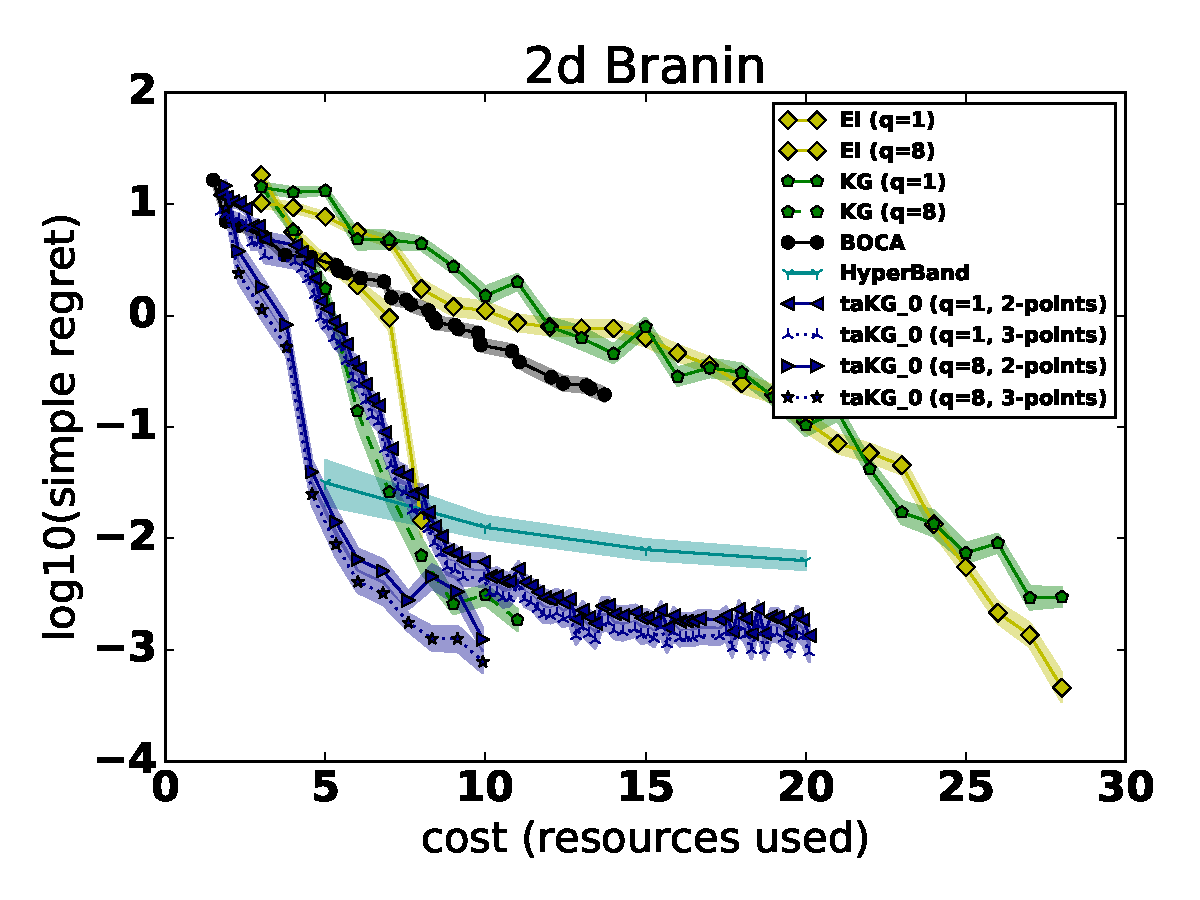
\includegraphics[width=\figwidth, height = \figheight]{fig/Branin.pdf}
  \subfigure
  \centering
  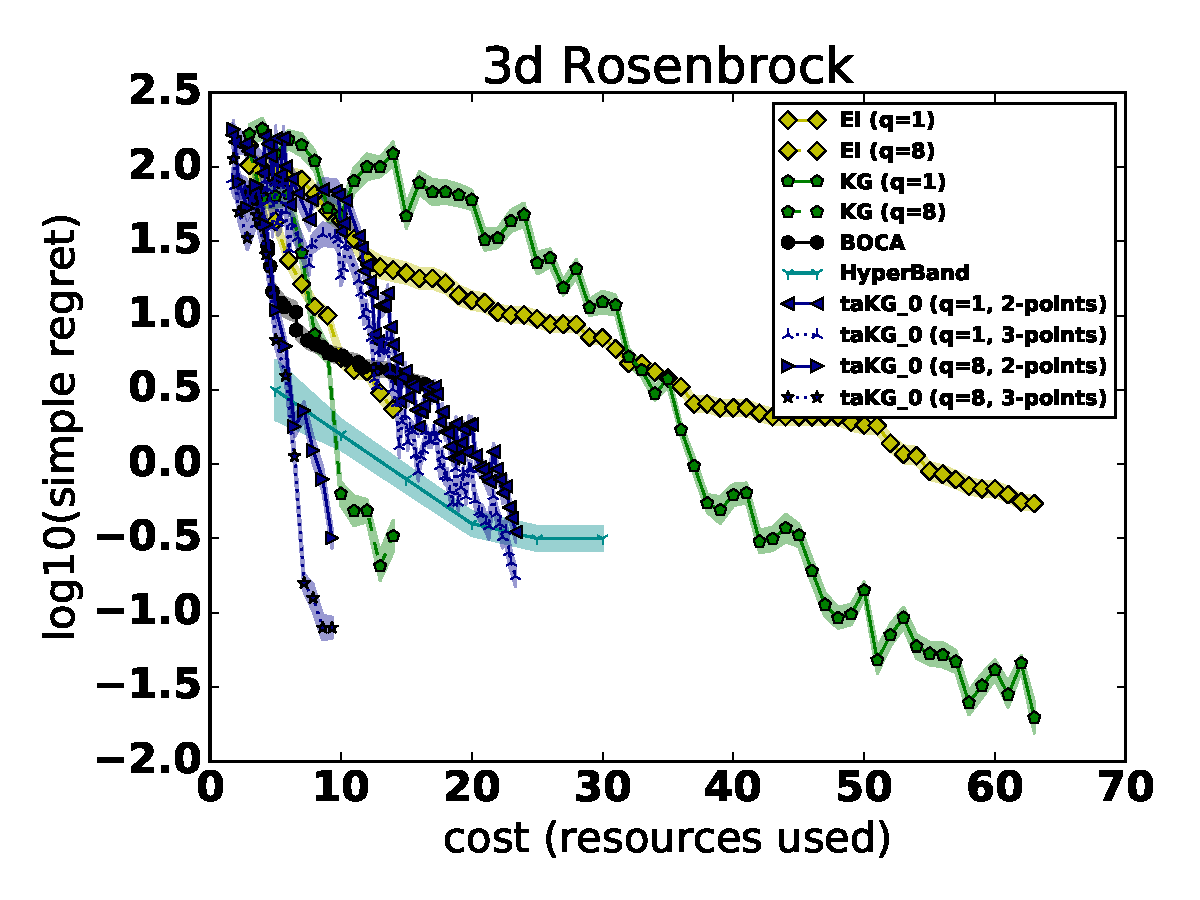
\includegraphics[width=\figwidth, height = \figheight]{fig/Rosenbrock.pdf}\\
    \subfigure
  \centering
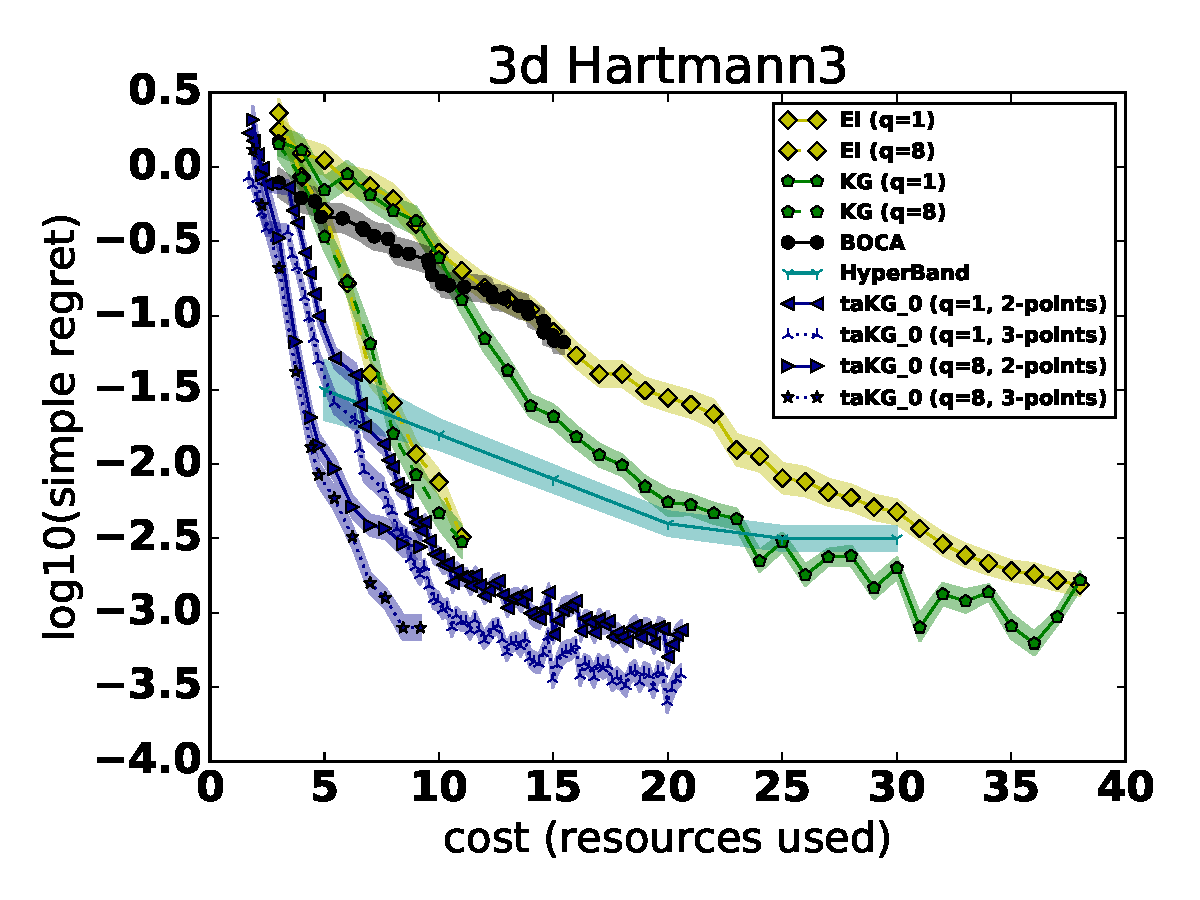
\includegraphics[width=\figwidth, height = \figheight]{fig/Hartmann3.pdf}
   \subfigure
  \centering
  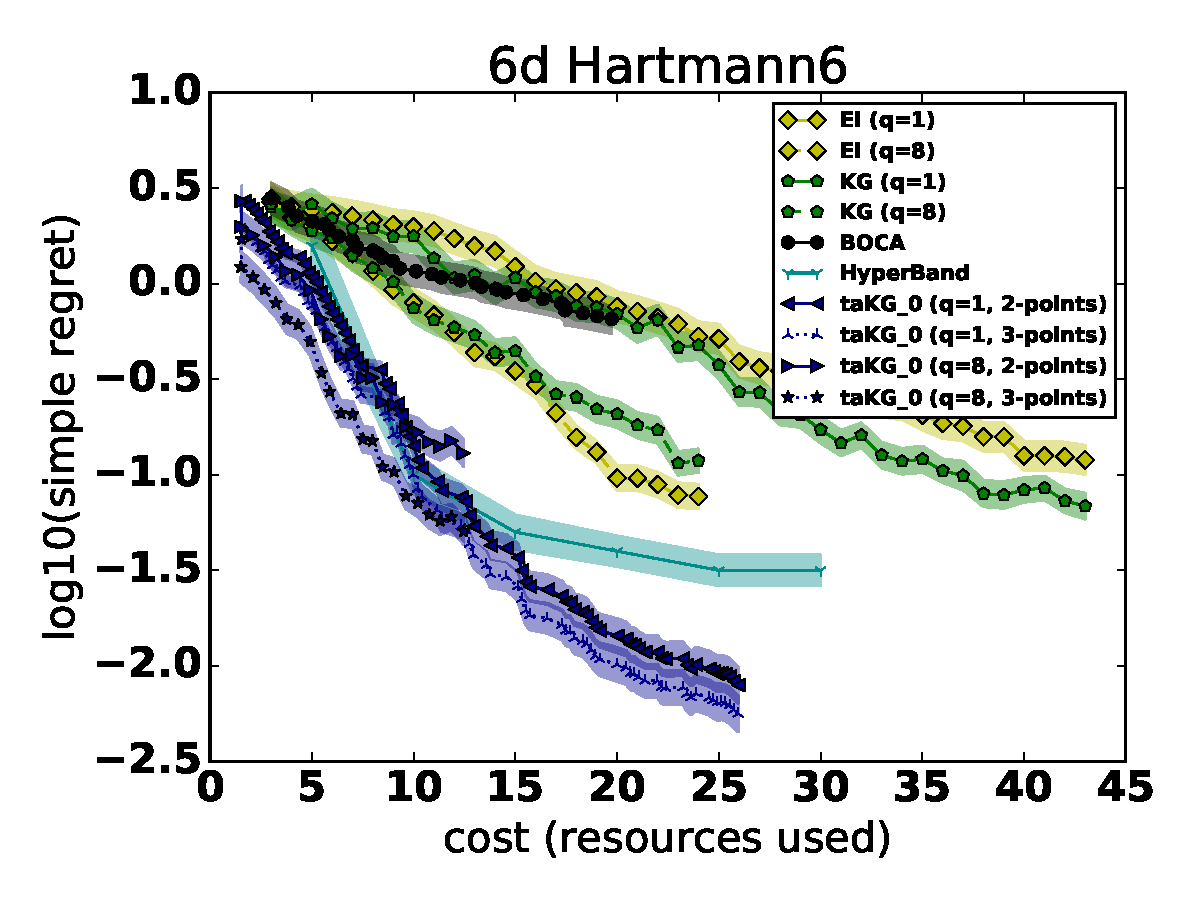
\includegraphics[width=\figwidth, height = \figheight]{fig/Hartmann6.pdf}
\vspace{-8pt}
\caption{\small Optimizing synthetic functions: Plots show simple regret over $40$ independent runs for synthetic functions with trace observations and one or two continuous fidelity controls for 2-d Branin, 3-d Rosenbrock, 3-d Hartmann, and 6-d Hartmann problems.  $q$ indicates batch size for fixed batch-size methods. $\taKG0$ outperforms competitors in both sequential and batch settings.}
\vspace{-12pt}
\label{Fig_syn_taKG}
\end{figure*}



Fig.~\ref{Fig_syn_taKG} shows results.  We run versions of $\taKGE$ using $|\S|$ set to $2$ (taKG\_0 2-points) and $3$ (taKG\_0 3-points).
Hyperband is implemented using values from \cite{li2016hyperband}: $R=1.01$, which is the maximum resource that can be consumed by a single fidelity; $\eta=3$, the default from Algorithm 1; and $s_{\max} = 4$, the value used in Table 1.

Sequential $\taKGE$ performs well relative to sequential competitors (EI, KG, BOCA) for both values of $|\S|$.
Batch $\taKGE$ with batch size 8 performs well relative to batch competitors (EI, KG, Hyperband).
(We consider Hyperband to be a batch method although the parallelism it leverages varies during its operation.)
Using the larger $|\S|$ improves the performance of $\taKGE$.

\subsection{Optimizing Hyperparameters of Neural Nets} \label{sect:hyperexp}
Here, we evaluate on hyperparameter optimization of neural networks. Benchmarks include the single-fidelity Bayesian optimization algorithms KG \citep{wu2016parallel} and EI \citep{jones1998efficient}, their batch versions, and the state-of-art hyperparameter tuning algorithms HyperBand and FaBOLAS.  

$\taKGE$ uses two fidelity controls: the training set size and the number of training iterations.  
FaBOLAS is specifically designed to use the training set size as its fidelity control.
We implement Hyperband also using the training set size as its fidelity (it can use only one fidelity).
We run Hyperband using the parameters described in \Section\ref{sect:synthetic}.  Because Hyperband did not perform as well as expected, we also performed experiments using $s_{\max} = 2$ and $s_{\max} = 1$.  $s_{\max} = 1$ is equivalent to random search, and is labeled so in plots.

Following \citet{li2016hyperband}, we set the cost to the number of training examples used in training, normalized by the number used in training with full fidelity. For example, if full fidelity uses $10^5$ training examples per epoch over $100$ epochs, then the cost of evaluating a set of hyperparameters using $10^4$ sub-sampled training examples per epoch over $10$ epochs is $10^4 \times 10 / (10^5 \times 100) = 0.01$. % Complete training has cost $1$.

\begin{figure*}[tb]
  \centering
  \subfigure
  \centering
  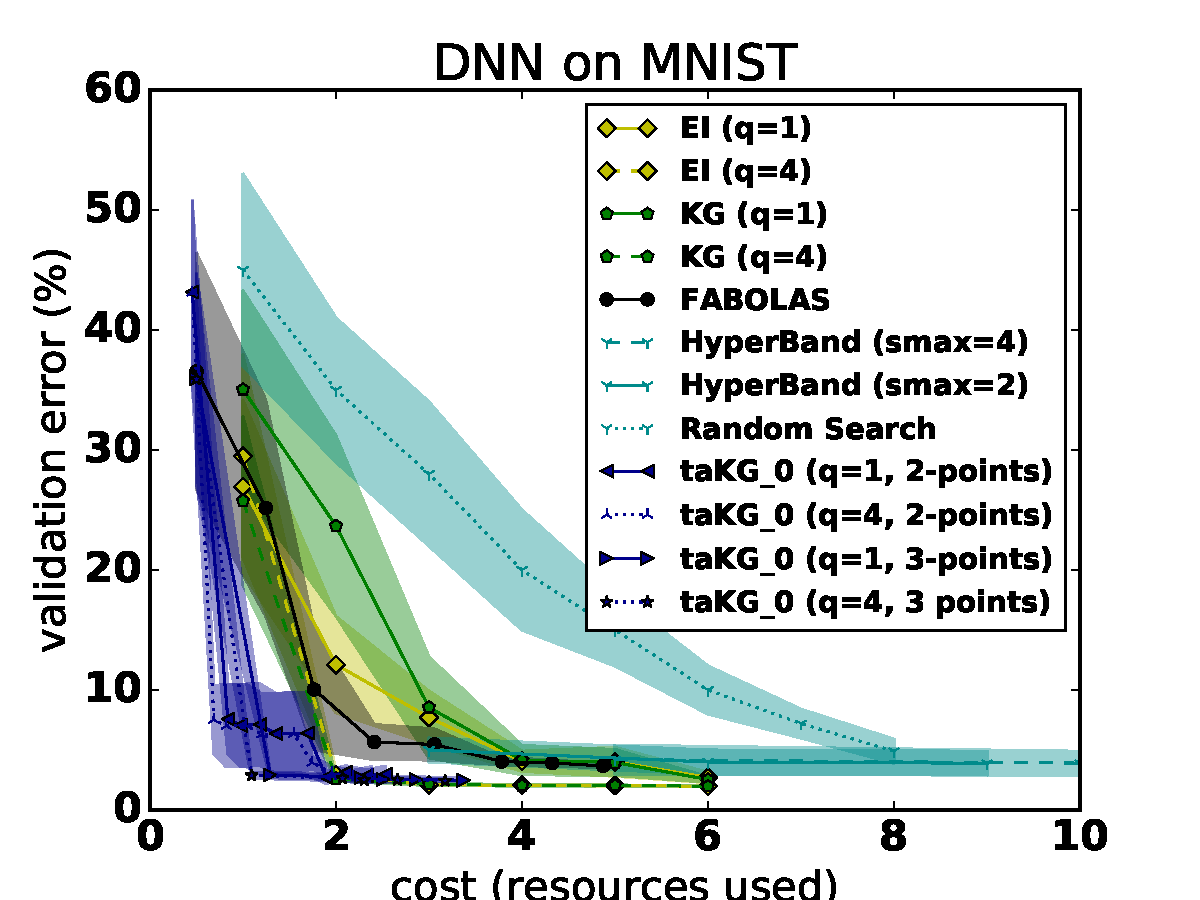
\includegraphics[width=\figwidth, height = \figheight]{fig/MNIST.pdf}
  \subfigure
  \centering
  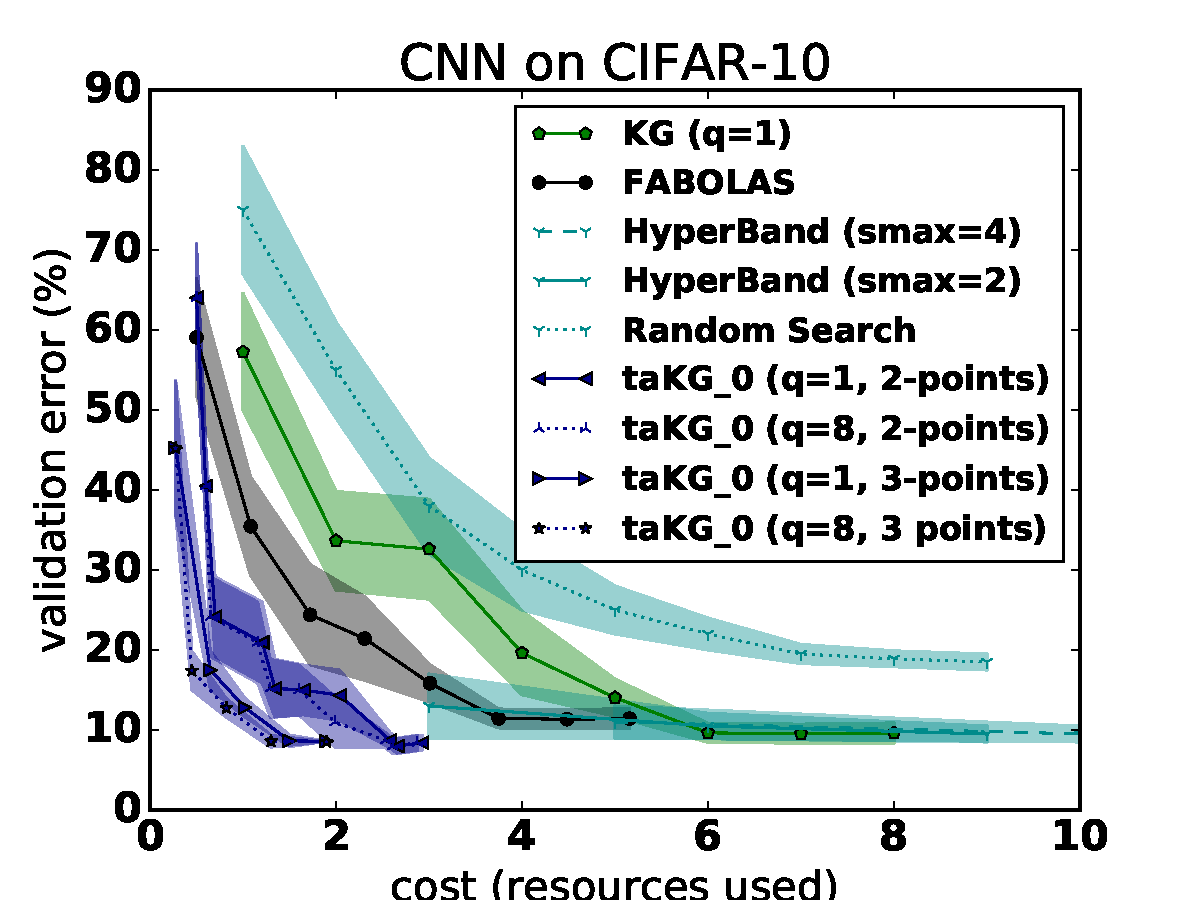
\includegraphics[width=\figwidth, height = \figheight]{fig/CIFAR10.pdf}\\
  \subfigure
  \centering
  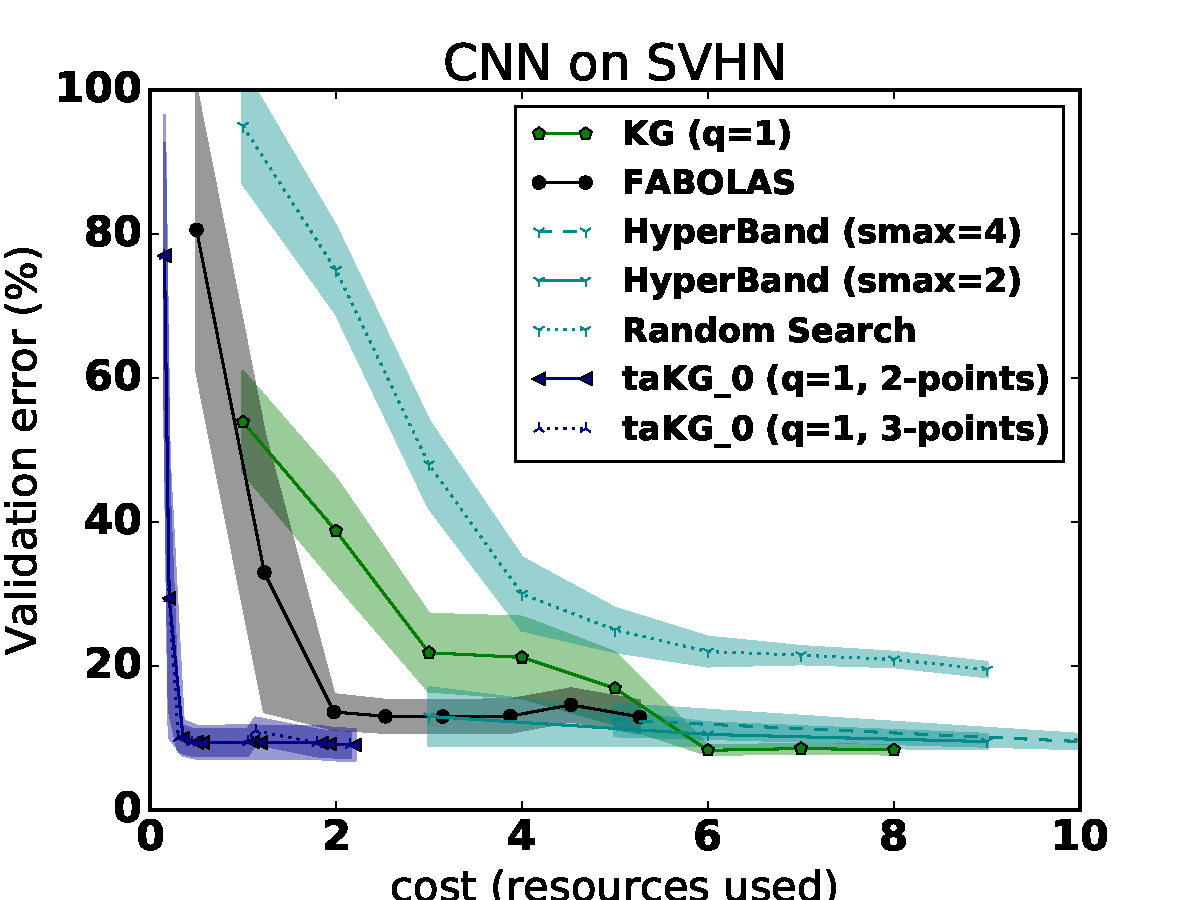
\includegraphics[width=\figwidth, height = \figheight]{fig/SVHN.pdf}
  \subfigure
  \centering
  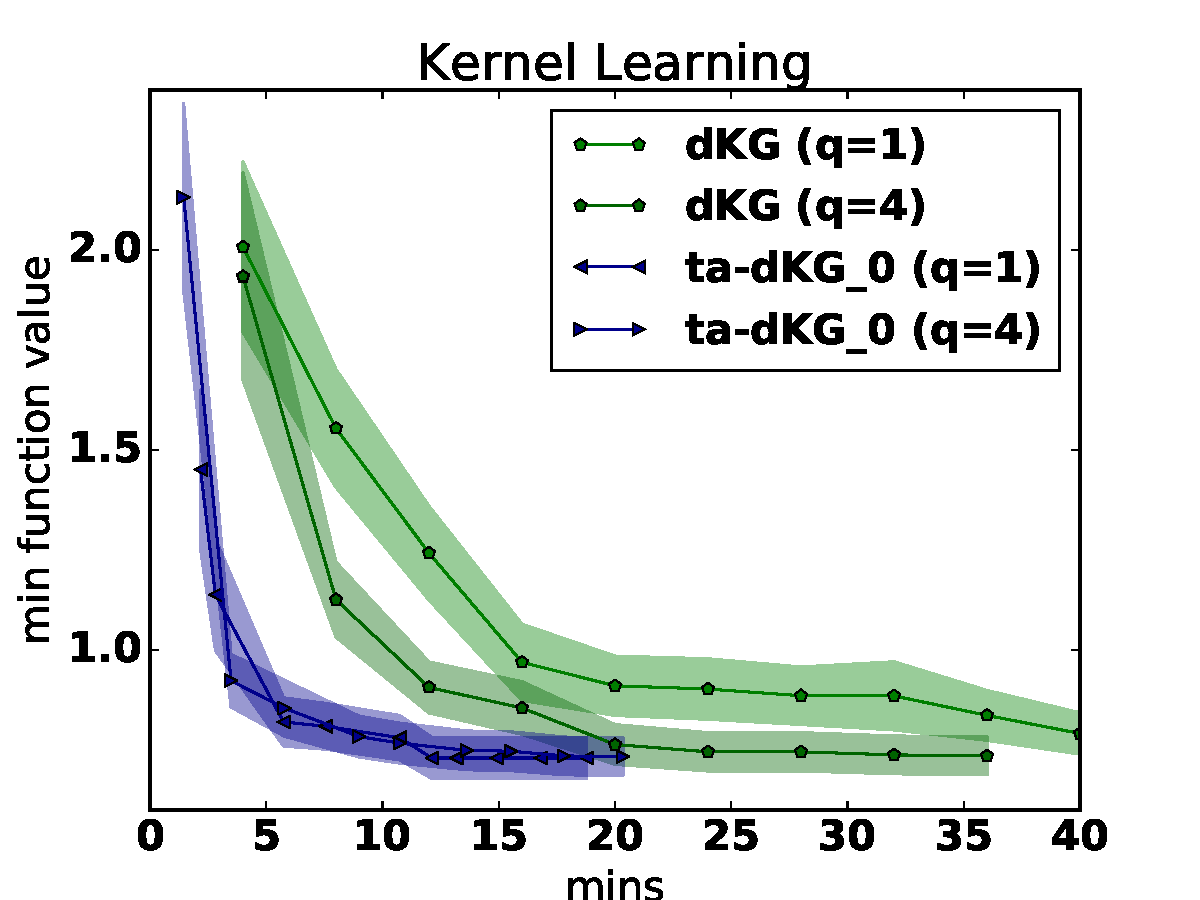
\includegraphics[width=\figwidth, height = \figheight]{fig/KISSGP.pdf}
\vspace{-8pt}
\caption{\small We show the validation error for tuning feedforward neural networks on MNIST (each with 20 runs); tuning convolutional neural networks on CIFAR-10 and SVHN (each with 10 runs); for KISS-GP kernel learning we show -log marginal likelihood divided by the number of datapoints.
$q$ indicates batch size for fixed batch-size methods. 
$\taKGE$ outperforms competitors in both sequential and batch settings.  }
\vspace{-12pt}
\label{Fig_deep_taKG}
\end{figure*}


\paragraph{Feedforward Neural Nets on MNIST}
\label{sect:mlps}
We tune a fully connected two-layer neural network on MNIST. The maximum number of epochs allowed is $20$. We optimize $5$ hyperparameters: learning rate, dropout rate, batch size and the number of units at each layer. 

Fig.~\ref{Fig_deep_taKG} shows that sequential $\taKGE$ outperforms the sequential methods KG, EI and the multi-fidelity hyperparameter optimization algorithm FaBOLAS. $\taKGE$ with batch size $4$ substantially improves over batch versions of KG and EI and the batch method Hyperband.

\paragraph{Convolutional Neural Nets on CIFAR-10 and SVHN}
\label{sect:cnns}
We tune convolution neural networks (CNNs) on CIFAR-10 and SVHN. Our CNN consists of 3 convolutional blocks and a softmax classification layer. Each convolutional block consists of two convolutional layers with the same number of filters followed by a max-pooling layer. There is no dropout or batch-normalization layer. We split the CIFAR-10 dataset into 40,000 training samples, 10,000 validation samples and 10000 test samples. We split the SVHN training dataset into 67,235 training samples and 6,000 validation samples, and use the standard 26,032 test samples. We apply standard data augmentation: horizontal and vertical shifts, and horizontal flips. We optimize $5$ hyperparameters to minimize the classification error on the validation set: the learning rate, batch size, and number of filters in each convolutional block. 
% XXX 
% Hyperband uses the size of the training set as its resource (it can use only one resource or fidelity), using a bracket size of $s_{\max} = 4$ as in \citet{li2016hyperband} and the maximum resource allowed by a single configuration set to 40000.
We set the maximum number of training epochs for all algorithms to $50$ for CIFAR-10 and $40$ for SVHN. 
Because of the computational expense of training CNNs, we leave out some benchmarks, dropping the single-fidelity method EI in favor of the structurally similar single-fidelity method KG, and performing batch evaluations for only some methods.

Fig.~\ref{Fig_deep_taKG} shows that sequential $\taKGE$ outperforms its competitors (including the batch method Hyperband) on both problems.  Using batch evaluations with $\taKGE$ on CIFAR-10 improves performance even further.
When we train using optimized hyperparameters on the full training dataset for $200$ epochs, test data classification error is $\sim12\%$ for CIFAR-10 and $\sim5\%$ for SVHN. 


\subsection{Optimizing Hyperparameters for Large-scale Kernel Learning}
\label{sect:kernel-learning}
We test derivative-enabled $\taKGE$ (ta-dKG$^\emptyset$) in large-scale kernel learning: the 1-d demo for KISS-GP \citep{wilson2015kernel} on the GPML website \citep{gpml}.  In this example, we optimize 3 hyperparameters (marginal variance, length scale, and variance of the noise) of a GP with an RBF kernel on $1$ million training points to maximize the log marginal likelihood. We evaluate both the log marginal likelihood and its gradient using the KISS-GP framework. We use two continuous fidelity controls: the number of training points and the number of inducing points.  We set the maximum number of inducing points to $m=1000$.

We compare ta-d-KG to the derivative-enabled knowledge gradient (d-KG) \citep{wu2017bayesian}, using both algorithms in the sequential setting and with a batch size of 4.  We leave out methods unable to utilize derivatives (including Hyperband and FaBOLAS), as these are likely to substantially underperform.
Fig.~\ref{Fig_deep_taKG} shows ta-dKG$^\emptyset$ finds a good solution faster than d-KG in sequential and batch settings.

%which dramatically improves the default hyperparameters set in the tutorial ($14\%$). The details of the optimized hyperparameters and the default hyperparameters are included in the appendix.


% used to be 125pt by 132 pt --- making a little smaller to save space
% If we have more room, can do 130x135

\section{CONCLUSION}
\label{sect:conclusion}
We propose a novel multi-fidelity acquisition function, the trace aware knowledge-gradient, that 
leverages special structure provided by trace observations,
is able to handle multiple simultaneous continuous fidelities, and 
generalizes to batch and derivative settings.
This acquisition function uses traces to outperform
state-of-the-art hyperparameter tuning algorithms.

% $\taKG$ and $\taKGE$, which generalize naturally to batch and derivative settings. $\taKGE$ 
%uses traces to
%find good hyperparameters for deep and kernel learning
%more quickly than state-of-art algorithms. 


\subsubsection*{Acknowledgements}
PIF was supported by NSF CAREER CMMI-1254298, NSF CMMI-1536895, and AFOSR FA9550-15-1-0038.
AGW was supported by NSF IIS-1563887, an Amazon Research Award and a Facebook Research Award.



\bibliographystyle{apalike}
\bibliography{pKG}


%References follow the acknowledgements.  Use unnumbered third level
%heading for the references title.  Any choice of citation style is
%acceptable as long as you are consistent.



\end{document}
